%!TEX root = ../master.tex
\chapter{Application Layer - Spring Boot \& Spring Cloud}
\label{appendix:application_layer}

This Appendix will provide an overview of the software used in the application layer within this present master thesis. 

\begin{figure}[H]
	\centering
	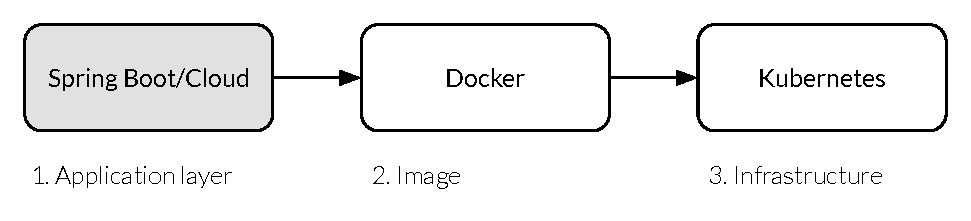
\includegraphics[width=12cm]{figures/technology_flow_spring}
	\caption{Application flow}
	\label{fig:flow_spring}
\end{figure}

\noindent There exist a lot of different frameworks for building microservices. A popular framework that lets you get started fairly quickly is Spring Boot and Spring Cloud. These two frameworks are chosen because of the rapidness of getting started. Another important reason is that Spring Boot runs great with Java. The 10 students of the 17 students answered Yes to the Votiee question about whether or not they have used Java.

\section*{What is Spring Boot?}

Spring Boot is a framework developed by Pivotal. It is designed to simplify bootstrapping and development of new Spring applications. Spring Boot takes an opinionated view of building production-ready Spring applications. It favors convention over configuration and is designed to get you up and running as quickly as possible. Spring Boot has evolved into what is defined as a chassis framework for microservices by Chris Richardson.\footnote{http://microservices.io/patterns/index.html} A microservice chassis framework helps you develop microservice applications fast. Spring Boot projects can easily be started via the Spring Initializr\footnote{http://start.spring.io}, which allows you to configure your project and set up dependencies. The Spring Boot framework can be used on the JVM with languages such as Java, Groovy, or Kotlin. 

\newpage
\section*{What is Spring Cloud?}

Spring Cloud builds on Spring Boot and provides developers a way to quickly build common patterns in distributed systems (e.g. configuration management, service discovery, circuit breakers, intelligent routing, micro-proxy, control bus, one-time tokens, global locks, leadership election, distributed sessions, cluster state).\footnote{http://projects.spring.io/spring-cloud/} 


\section*{Spring Cloud Netflix OSS}
Spring Cloud Netflix provides Netflix OSS integrations for Spring Boot apps through autoconfiguration and binding to the Spring Environment. Netflix Open Source Software Center (Netflix OSS) is the source for Netflix services. Netflix has been a huge contributor to the open source environment, and many to the tools used at Netflix are open sourced and can easily be integrated into your applications. Spring Cloud Netflix enables you to quickly enable and configure Netflix OSS software by applying a few simple annotations. Some of the patterns used within this present master thesis includes, Circuit Breaker (Hystrix), Intelligent Routing (Zuul), HTTP Rest client (Feign).

\section*{Zuul - API Gateway}
The first Netflix OSS component we will discuss is the Netflix's implementation of the API Gateway pattern, namely Zuul. Before going into the details of Zuul, we will first describe what the API Gateway pattern is. The pattern is described by Chris Richardson.\footnote{http://microservices.io/patterns/apigateway.html}
 
\subsection*{The API Gateway Pattern}
\subsubsection*{Context}  
Building a microservice architecture, you have multiple clients communicating with your backend. The clients communicate with individual services and thereby have to communicate with many different services to aggregate the data internally upon reception of responses from these services

\subsubsection*{Problem}  
How do clients minimize the number of request to the backend, e.g. reduce these chatty interfaces? and how to allow clients to communicate with individual services in a microservice based application?

\subsubsection*{Forces}  
Chris Richardsen describes some of the many forces as follows:
\begin{itemize}
    \setlength\itemsep{0.05em}
  \item Granularity of APIs provided by microservices is often different than what a client needs
  \item Different clients need different data
  \item Network performance is different for different types of clients
  \item The number of service instances and their locations (host+port) changes dynamically
  \item Partitioning into services can change over time and should be hidden from clients
\end{itemize}


\subsubsection*{Solution}
The solution is to implement a server-side aggregation endpoint or API gateway. The API Gateway is responsible for aggregating data or in some cases acts as a simple routing layer for appropriate services. The API gateway can be seen as a single point of failure, or as Sam Newman describes it as a \textit{single monolithic gateway}. A better approach may be to create multiple API gateways for the different platform or frontends that your application needs to support. This is also referred to as \textit{backends for frontends}.

\begin{figure}[H]
	\centering
	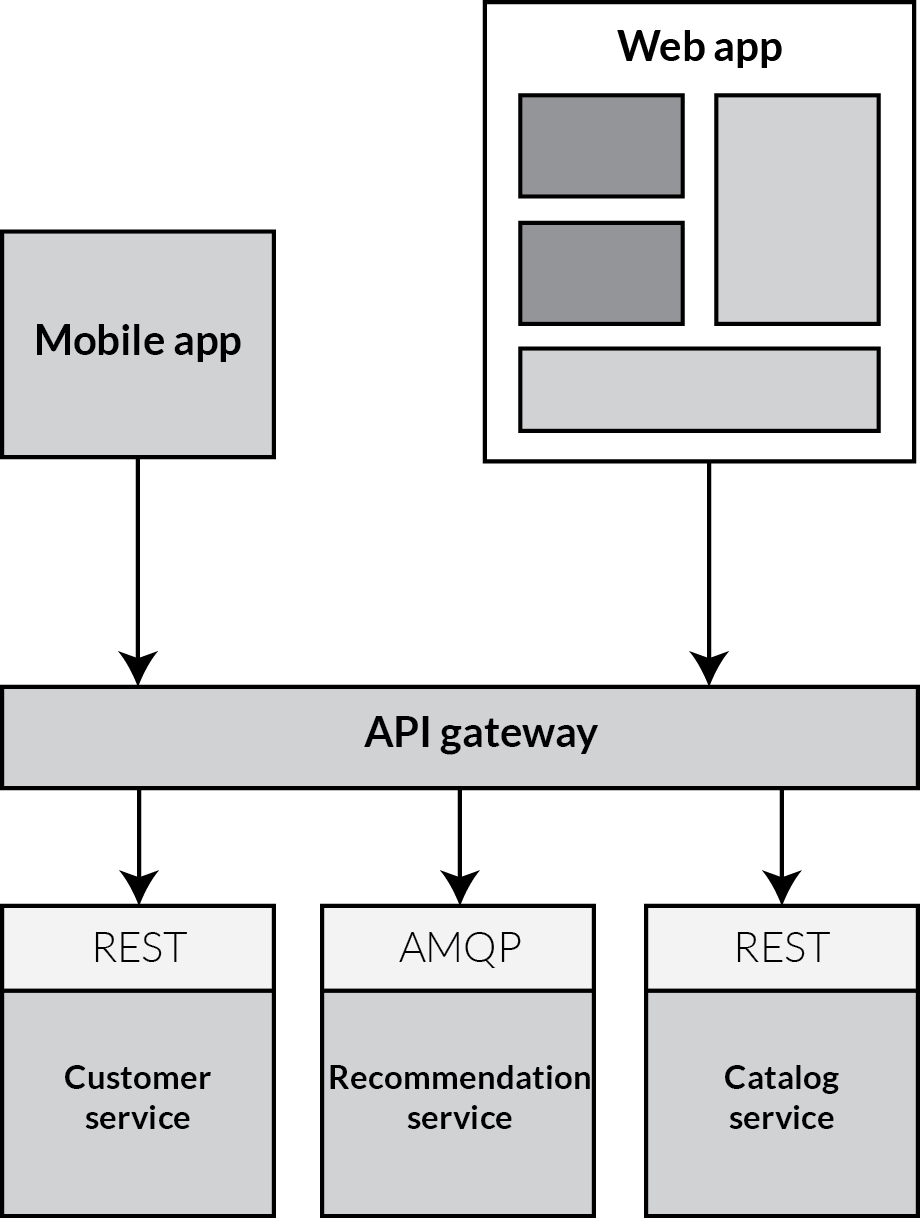
\includegraphics[width=8cm]{figures/api_gateway}
	\caption{Pattern: API Gateway}
	\label{fig:api_gateway}
\end{figure}

\subsubsection*{Resulting Context}   
\textbf{\textit{Benefits:}}
\begin{itemize}
    \setlength\itemsep{0.05em}
  \item Clients are isolated from the partitioning of the microservice architecture behind the gateway
  \item Clients do not have to worry about locations of specific services
  \item Reduces the number of requests/roundtrips
  \item Simplifies the clients by moving the aggregation logic into the API gateway
\end{itemize}

\noindent\textbf{\textit{Drawbacks:}}
\begin{itemize}
    \setlength\itemsep{0.05em}
  \item Increased complexity - API gateway is one more added to the list of moving parts within you microservices architecture
  \item Increased response time compared to direct calls, because of the additional network hop through the API gateway
  \item Danger of implementing to much logic in the aggregation layer
\end{itemize}

\subsection*{Zuul}
To implement the API Gateway pattern in Spring Cloud we use the Netflix OSS component, Zuul. Zuul makes the process of implementing this pattern easy. In your main application file, a simple annotation @EnableZuulProxy has to be added 

\begin{lstlisting}[language=Java]
@SpringBootApplication
@EnableZuulProxy
public class ApiGatewayApplication {

    public static void main(String[] args) {
        SpringApplication.run(ApiGatewayApplication.class, args);
    }
}
\end{lstlisting}

\noindent Besides this simple annotation, we need to apply some configuration on what Zuul has to do when it receives a request. This can be configured in application.properties file by adding the following:

\begin{lstlisting}
zuul.routes.book.path=/movies/**  
zuul.routes.book.url=http://localhost:9000  
ribbon.eureka.enabled=false  
server.port=8080  
\end{lstlisting}

\noindent This tells Zuul, that whenever a request is received at localhost:8080/movies, Zuul will route this request to a microservices running at localhost:9000/movies. \\

\noindent This was a high-level overview of how Zuul can be used, Zuul can be configured in many ways. In a production environment Zuul can act as the gatekeeper to the rest of your microservices backend by handling authentication, etc. 

\noindent Our blog contain a more detailed description of how to setup Zuul, and example respository is also provided: \url{http://rpi-cloud.com/apigatewaypattern/}

\section*{Spring Cloud Config}

Changing configurations on running services can be cumbersome, especially if the application does not have a way to be configured remotely. Spring Cloud Config provides a way to make this easier by introducing a Config Server from which clients fetch their configuration. The figure below illustrates how Spring Cloud Config works.

\begin{figure}[H]
	\centering
	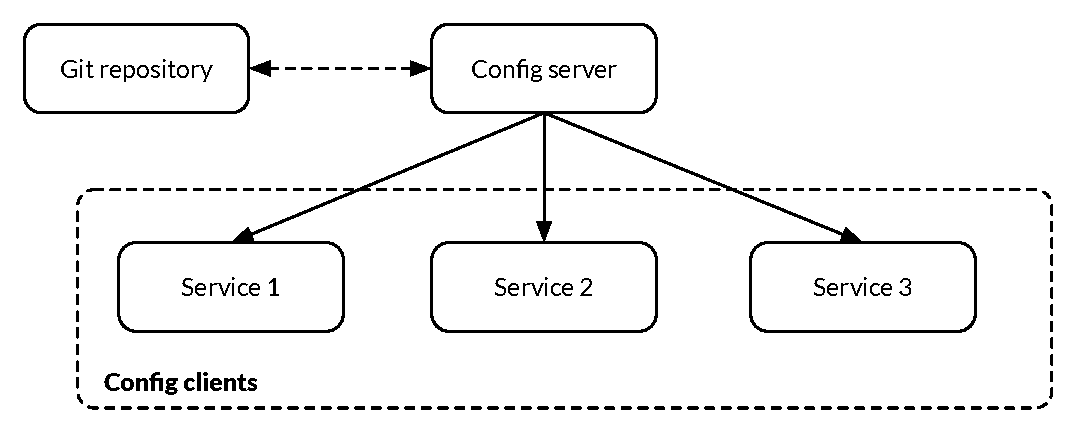
\includegraphics[width=11cm]{figures/config_server}
	\caption{Pattern: API Gateway}
	\label{fig:api_gateway}
\end{figure}

\begin{itemize}
  \item The Git repository is used to store the configuration since Git is pretty good at tracking and storing changes.
  \item The Config server keeps itself up to date with the Git repository, and serves HTTP requests with configurations for the clients.
  \item The Config clients request the configuration from the config server, which sets the properties in the application.
\end{itemize}

\noindent Spring Cloud Config provides server and client-support for externalized configurations in distributed systems. An integrating this pattern into your applications is fairly simple.

\subsubsection*{Config Server}
First we need to setup a Config server as a separate service. This can easily be done using the before mentioned Spring Initializr\footnote{http://start.spring.io}. The Config server has to point to the Git repository where the configurations are stored. This is configured in the bootstrap.yml file as shown below:

\begin{lstlisting}
spring:  
  application:
    name: config-service
  cloud:
    config:
      server:
        git:
          uri: https://github.com/rpicloud/guide-cloud-config
server:  
  port: 8888
\end{lstlisting}

\subsubsection*{Config Clients}
The config clients has to be configured to point to the Config Server. This is easily done in the bootstrap.yml file of the client as follows:


\begin{lstlisting}[]
spring:  
  application:
    name: configclient
  cloud:
    config:
      uri: http://localhost:8888
\end{lstlisting}

\noindent This is all that is needed to setup the Spring Cloud Config pattern. This pattern allows us to have a central place to manage external properties of our applications across all environments. 

\noindent A blog post explaining the setup in more detail can be found on our blog: \url{http://rpi-cloud.com/guide-spring-cloud-config/}.


\section*{Hystrix - Circuit Breaker}

Hystrix is Netflix's implementation of the Circuit Breaker pattern. Hystrix makes it easy to apply timeouts, add the circuit breaker pattern with fallback methods, and further it provides a dashboard for monitoring these integration points as well. To enable Hystrix a few simple annotations is needed, @EnableCircuitBreaker, and @EnableHystrixDashboard if the dashboard is needed. This is shown below.

\lstinputlisting[language=java,label={lst:hystrix_enable}, caption={Enabling Hystrix}]{scripts/hystrix_enable.java}

\noindent To implement a fallback method for when the circuit is open, i.e. the integrating service is down, a simple annotation is added to the method as shown below:

\lstinputlisting[language=java,label={lst:hystrix_apply}, caption={Implementing Hystrix}]{scripts/hystrix.java}

\noindent As shown in Listing~\ref{lst:hystrix_apply} the @HystrixCommand takes a fallback method as an argument. In the example we provide a method called open, to simply return an array of backup data which in this case is a list of strings.

\noindent In the code example shown in Listing~\ref{lst:hystrix_apply}, Feign is used as a Rest Client builder. Feign is a declarative web service client that makes writing web service clients easier. Further it integrates easily with other Netflix tools, and also with already available components like the JacksonDecoder. 